Pour guider la définition de notre méthode nous avons identifié
plusieurs principes que nous voulons voir respectés.

\subsection{Intégration dans le contexte métier}

Le premier des principes que nous voulons voir respecté par notre
méthodologie est celui de sa bonne intégration dans le contexte
métier.
%
C'est un point que nous avons déjà évoqué a plusieurs reprises. Nous
souhaitons que notre méthode soit conçue dans l'optique de son
application finale, \ie que nous avons à cœur de réfléchir à son
appropriation et son développement par les secouristes. Pour autant
nous ne souhaitons pas sacrifier la généricité de notre méthode, c'est
pourquoi son développement relève d'un équilibre entre la généricité
de la méthode et la spécificité de certains paramétrages.

\subsubsection{\texttt{Le secouriste comme super joker + ZIR}}

Parmi les choix visant à faciliter l'intégration de notre méthode il y
en a un dont nous avons déjà parlé, le rôle du secouriste. En effet,
comme nous l'indiquions dans la première partie, nous ne souhaitons
pas que notre méthode se substitue au secouriste, mais au contraire
qu'elle l’assiste. Ce choix (tout du moins tel que présenté dans le
\autoref{chap:01}) est hérité d'une décision faite au sein du projet
CHOUCAS dans son ensemble, celle de ne pas travailler sur
l'interprétation automatisée du requérant, nécessitant dès lors un
intermédiaire, le secouriste, entre le combiné téléphonique et
l'interface.

\begin{figure}
  \centering
  % \input{../figures/diag_activ_secours.tex}
  \caption{dcsqd}
  \label{fig:diag_acti_secours}
\end{figure}

L'interaction avec le secouriste nous permet également de disposer
d'une \emph{zone initiale de recherche} (ZIR, \cite{Viry2019}),
délimitant la zone où la présence de la victime est, selon le
secouriste, certaine. La définition d'une telle zone est un préalable
indispensable à la \emph{spatialisation} des \emph{indices de
  localisation.}
%
car de grandes régions peuvent appartenir à la zone de
localisation compatible spatialisée, pour peu que l'a
%
lorsque ces derniers se référent à des objets
indéfinis (\eg \enquote{un lac}, \enquote{une ville}, \enquote{un
  sommet}) tous les objets de ce type doivent êtres considérés, aucune
autre information ne permettant d'en raffiner la sélection. Cette
première saisie nous permet de restreindre la zone de recherche de la
victime, qui, en l'absence de cette information ne peut-être que
l'ensemble de la zone d'intervention de l'\ac{usem} contactée.

\subsubsection{La modélisation explicite des connaissances}

Les phases de spatialisation et de fusion différent par un point
essentiel. La fusion consiste à regrouper diddérentes zones de
localisaiton compatibles dans le but de construire une seule zone de
localisation probable. Par conséquent, tous les individus en entrée de
cette opération sont de la même nature, \ie des objets
géographiques. L'opération de fusion ne nécessite donc pas la
définition de comportements particuliers, adaptés à des cas qui le
sont tout autant. La spatialisation par contre nécessite le
développement d'une méthode adaptée à chaque \emph{relation de
  localisation.} En effet on spatialise pas la \emph{relation}
\enquote{sous} de la même manière que la \emph{relation}
\enquote{entre}. Il est donc nécessaire de définir une méthode de
\emph{spatialisation} pour chaque \emph{relation de localisation} et
d'en proposer une implémentation. Une possibilité serait d'écrire des
fonctions \emph{ad hoc} lors de l'implémentation et de les détailler
ici. Ce faisant l'ensemble des connaissances produites lors de
l'élaboration des méthodes de spatialisation se retrouverait dans le
code, ce qui ne faciliterait pas la compréhension et l'utilisation
appliquée de notre travail.

Pour faciliter l'intégration de notre travail dans le contexte métier
du secours en montagne nous avons choisi d'adopter une démarche
imposant la modélisation explicite des connaissances. Cette démarche
est inspirée des \emph{systèmes à base de connaissances} où ces
dernières sont formalisées au sein d'une ontologie lue et interprétée
par le code. Ainsi, on peut imaginer que les règles de
\emph{spatialisation} de toutes les \emph{relations de localisations}
soient formalisées dans une ontologie des \emph{ad hoc,} lisible et
modifiable à chaque instant. Cette approche offre plusieurs
avantages. D'une part, comme énoncé précédemment elle permet aux
utilisateurs de nos méthodes de \emph{spatialisation} de disposer
d'une forme d'auto-documentation, permise par la centralisation de
toutes les règles de spatialisation. Cette centralisation facilite
également la modification où l'ajout de règles de
\emph{spatialisation.} De plus cette ontologie peut être exploitée et
diffusée séparément.

\subsection{Principes de modélisation}

\subsubsection{Décomposition des \emph{relations de localisation}}

Comme nous l'indiquions précédemment (cf. \ref{subsec:2-1-1}) une même
\emph{relation de localisation} peut voir sa sémantique varier en
fonction de son contexte d'utilisation \autocite[16]{Borillo1998}.
C'est par exemple le cas de la relation de localisation
\enquote{\emph{sous}}. On peut être \enquote{sous \emph{un pont}} ou
\enquote{sous \emph{une route}}. Or la sémantique de ces deux exemples
diffère quelque peu. Le premier cas sous-entend un \emph{recouvrement}
(\ie \emph{le pont est entre le locuteur et le ciel}) alors que ce
n'est pas le cas pour le second. Cette différence s'explique par la
nature des objets de référence. On peut être recouvert par \emph{un
  pont} (ou un arbre, le ciel, \emph{etc.})  mais pas par une route
(ou un bâtiment). Ainsi il est nécessaire d'identifier ces différences
sémantiques pour pouvoir \emph{spatialiser} une \emph{relation de
  localisation.}
%
On pourrait augurer que, du fait de leur différence sémantique, ces
deux exemple d'utilisation du \enquote{\emph{sous}} correspondent en
réalité à deux \emph{relations de localisation} différentes, mais
désignées par la même \emph{préposition spatiale.}
%
Ces deux \emph{relations de localisation} ont cependant un point
commun, qui justifie l'utilisation de la même préposition, leur
\emph{sujet} est situé à une altitude inférieure à celle de
\emph{l'objet de référence.} Ce sont ces régularités sémantiques que
nous proposons d'exploiter \autocite{Bunel2019a}.

Pour ce faire, nous proposons de décomposer les \emph{relations de
  localisation} en un ensemble de \emph{relations de localisation
  atomiques} que nous aurons préalablement identifiées et explicitées,
conformément au \emph{principe de modélisation explicite des
  connaissances.} Chaque relation de \emph{localisation atomique}
correspondant alors à une composante sémantique indépendante. Par
exemple la \emph{relation de localisation} \enquote{\emph{sous}}, dans
l'indice de localisation \enquote{je suis \emph{sous} un pont}
pourrait être décomposée en plusieurs \emph{relations de localisation
  atomiques} une première indiquant que le \emph{sujet} est situé à
une altitude inférieure de \emph{l'objet de référence} et une seconde
indiquant que le \emph{sujet} est recouvert par \emph{l'objet de
  référence.} La décomposition de la \emph{relation de localisation}
conduit à construire deux nouveaux \emph{indices de localisation,} qui
ne diffèrent que par leur \emph{relation de localisation.} On peut
alors \emph{spatialiser} \emph{l'indice de localisation} en combinant
les \emph{spatialisations} des \emph{relations de localisations
  atomiques.} Par exemple, si l'on cherche à modéliser l'\emph{indice
  de localisation} \enquote{je \emph{suis sous} un pont} on pourra
construire la \emph{zone de localisation} correspondant à
\emph{l'indice de localisation} \enquote{je suis \emph{recouvert} par
  un pont} et la \emph{zone de localisation} correspondant à
\emph{l'indice de localisation} \enquote{je suis \emph{à une altitude
    inférieure} à un pont}, puis les combiner à l'aide d'un opérateur
de fusion \emph{ad hoc,} pour obtenir la \emph{zone de localisation
  compatible} correspondant à \emph{l'indice de localisation}
\enquote{je suis \emph{sous} un pont}.

\begin{figure}
  \centering
  \caption[Illustration de la décomposition d'un \emph{indice de
    localisation}]{Décomposition de \emph{l'indice de localisation:}
    \enquote{Je suis sous une ligne électrique}}
  \label{fig:dec_sous}
\end{figure}

Cette approche a pour objectif et intérêt principal de permettre
l'exploitation des récurrences sémantiques que l'on peut trouver entre
différentes \emph{relations de localisation.} Par exemple, la notion
de \emph{proximité} est à la base de nombreuses \emph{relations de
  localisation} comme \enquote{\emph{à côté}}, \enquote{\emph{aux
    alentours de}}, \enquote{\emph{devant}}, \emph{etc.} En
définissant une méthode de \emph{spatialisation} de cette
\emph{relation de localisation atomique} il devient possible de la
réutiliser et de la combiner à d'autres \emph{relations de
  localisation atomiques} permettant ainsi de modéliser un grand
ensemble de \emph{relations de localisations.}

On peut cependant s'attendre à ce que plusieurs \emph{relations de
  localisation} ne soient pas décomposables en un ensemble de
\emph{relations de localisation atomiques.} C'est par exemple le cas
de la notion de \emph{proximité} qui peut être employée
indépendamment, comme dans la phrase \enquote{je suis proche d'un
  supermarché}. Ainsi certaines \emph{relations de localisation} sont
des \emph{relations atomiques,} non décomposables.

\tdi{Ajouter le principe de décomposition des objets ?}

\subsubsection{Autonomie de la \emph{spatialisation}}

Un autre principe que nous souhaitons développer est celui de la
séparation maximale des étapes du processus.

Comme nous l'expliquions dans le \autoref{chap:2} deux étapes sont
nécessaires pour transformer une position décrite en une \emph{zone de
  localisation probable,} la \emph{spatialisation} et la
\emph{fusion.} Mais ces deux étapes peuvent être combinées
différemment.

Une première solution consiste à \enquote{chainer} la
\emph{spatialisation} des différents \emph{indices de localisation,}
comme on peut le voir sur la figure \ref{fig:comp_approches_lin}. Avec
cette approche les différentes \emph{zones de localisation
  compatibles} sont créées les unes à la suite des autres, ainsi la
zone de recherche en entrée de chaque étape de \emph{spatialisation}
dépend des \emph{spatialisations} précédentes. Avec cette approche,
l'opération de \emph{fusion} est implicite, elle s'opère, en partie, à
chaque nouvelle \emph{spatialisation,} puisque les zones ne
correspondant pas aux \emph{indices de localisation} sont retirées peu
à peu. La \emph{zone de localisation probable} (en bleu sur la figure
\ref{fig:comp_approches}) est obtenue une fois que l'on a
\emph{spatialisé} tous les \emph{indices de localisation.} Cette
approche est la première que nous ayons envisagée. Elle a pour
avantage d'être simple à concevoir et à développer. Cependant cette
approche à un problème majeur. À cause de l'enchainement des étapes de
\emph{spatialisation} les erreurs se répercutent d'une étape à
l'autre. Ainsi, si un des \emph{indices de localisation} est mal
\emph{spatialisé}, que ce soit à cause de la méthode utilisée ou d'une
mauvaise description, cela se répercute sur toutes les
\emph{spatialisations} ultérieures. La moindre correction impose donc
de refaire l'ensemble des traitements.

Une seconde solution, plus robuste, consiste à effectuer l'ensemble
des opérations de \emph{spatialisation} en parallèle, comme le montre
la figure \ref{fig:comp_approches_sep}. Avec cette approche la
\emph{spatialisation} des différents \emph{indices de localisation}
est effectuée séparément et leur \emph{fusion} est effectuée dans un
second temps. Comme pour la démarche \enquote{chainée} une
\emph{spatialisation} erronée peut impacter la \emph{zone de
  localisation probable,} toutefois il est plus facile de corriger ces
erreurs. En effet, si les différentes \emph{zones de localisation
  compatibles} ont été conservées il est possible de faire une
nouvelle \emph{fusion} en retirant un, ou plusieurs \emph{indices de
  localisation.} Alors qu'avec une approche \enquote{chainée} il est
nécessaire de refaire toutes les opérations de \emph{spatialisations}
ultérieures à celle de \emph{l'indice de localisation} que l'on
souhaite modifier ou retirer et ce même si les résultats
intermédiaires ont été conservés.

\begin{figure}
  \centering
  \subfloat[Construction suivant une démarche linéaire]{
    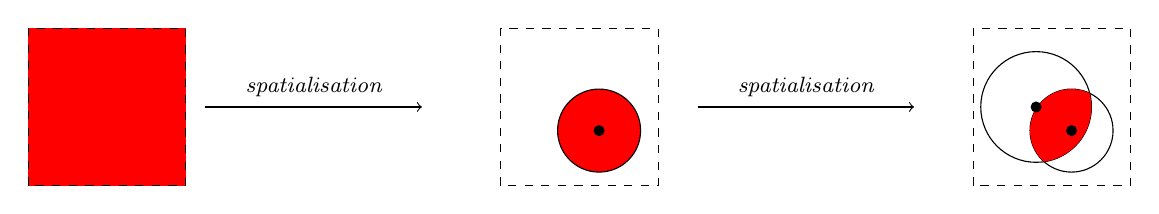
\begin{tikzpicture}

  \begin{scope}
    \path[fill=red] (0,0) rectangle (2,2);
	\path[draw, dashed] (0,0) rectangle (2,2);
  \end{scope}

  \path[draw, ->] (2.25,1) --++ (2.75,0)  node[pos=.5, above] {\footnotesize \itshape spatialisation};

  \begin{scope}[xshift=6cm]
	\path[draw, dashed] (0,0) rectangle (2,2);
	\begin{scope}
	    \begin{scope}
	      \clip (0,0) rectangle (2,2);
	      \fill[red] (1.25,.7) circle [radius=15pt];
	      \path[draw] (1.25,.7) circle [radius=15pt];
	    \end{scope}
	\end{scope}
    \node[circle, inner sep=0pt,minimum size=4pt, fill] (c) at (1.25,.7)
    {};
  \end{scope}



  \path[draw, ->] (8.5,1) --++ (2.75,0)  node[pos=.5, above] {\footnotesize \itshape spatialisation};




  \begin{scope}[xshift=12cm]
	\path[draw, dashed] (0,0) rectangle (2,2);
	\path[draw] (1.25,.7) circle [radius=15pt];
    \path[draw](.8,1) circle [radius=20pt];
	\begin{scope}
	    \begin{scope}
	      \clip (1.25,.7) circle [radius=15pt];
	      \fill[red] (.8,1) circle [radius=20pt];
	    \end{scope}
	\end{scope}
    \node[circle, inner sep=0pt,minimum size=4pt, fill] (c) at (1.25,.7)
    {};
    \node[circle, inner sep=0pt,minimum size=4pt, fill] (c) at (.8,1)
    {};
  \end{scope}


\end{tikzpicture}
    \label{fig:comp_approches_lin}
  }

  \subfloat[Construction suivant une démarche autonome]{
    \begin{tikzpicture}

  \begin{scope}
    \path[ffa] (0,0) rectangle (2,2);
    \path[ffc] (0,0) rectangle (2,2);
  \end{scope}

  \path[draw, ->] (2.25,1) --++ (2.75,1.5)  node[pos=.5, above] {\footnotesize \itshape spatialisation};
  \path[draw, ->] (2.25,1) --++ (2.75,-1.5)  node[pos=.5, above] {\footnotesize \itshape spatialisation};

  \begin{scope}[xshift=6cm, yshift=-1.5cm]
    \path[draw, dashed] (0,0) rectangle (2,2);
    \begin{scope}
      \begin{scope}
        \clip (0,0) rectangle (2,2);
        \fill[ffa] (1.25,.7) circle [radius=15pt];
        \path[ffc] (1.25,.7) circle [radius=15pt];
      \end{scope}
    \end{scope}
    \node[circle, inner sep=0pt,minimum size=4pt, fill] (c) at (1.25,.7)
    {};
  \end{scope}

  \begin{scope}[xshift=6cm,yshift=1.5cm]
    \path[draw, dashed] (0,0) rectangle (2,2);
    \fill[ffa](.8,1) circle [radius=20pt];
    \path[ffc](.8,1) circle [radius=20pt];
    \node[circle, inner sep=0pt,minimum size=4pt, fill] (c) at (.8,1)
    {};
  \end{scope}

  \path[draw, ->] (8.5,1) --++ (2.75,0)  node[pos=.5, above] {\footnotesize \itshape fusion};


  \begin{scope}[xshift=12cm]
    \path[draw,dashed] (0,0) rectangle (2,2);
    \path[draw,dashed] (1.25,.7) circle [radius=15pt];
    \path[draw,dashed](.8,1) circle [radius=20pt];
    \begin{scope}
      \begin{scope}
        \clip (1.25,.7) circle [radius=15pt];
        \fill[ffa2] (.8,1) circle [radius=20pt];
        \path[ffc2] (.8,1) circle [radius=20pt];
      \end{scope}
      \begin{scope}
        \clip (.8,1) circle [radius=20pt];
        \path[ffc2] (1.25,.7) circle [radius=15pt];
      \end{scope}
    \end{scope}
    \node[circle, inner sep=0pt,minimum size=4pt, fill] (c) at (1.25,.7)
    {};
    \node[circle, inner sep=0pt,minimum size=4pt, fill] (c) at (.8,1)
    {};
  \end{scope}


\end{tikzpicture}
    \label{fig:comp_approches_sep}
  }
  \caption{Comparaison du processus de construction de la \emph{zone
      de localisation probable} pour une alerte à deux \emph{indices
      de localisation}.}
  \label{fig:comp_approches}
\end{figure}

Le principe de modélisation autonome peut, de plus, tirer parti du
principe de décomposition précédemment présenté.

% Justifier choix

\subsection{Principes sémantiques}

\subsubsection{Modélisation non bivalente}
\texttt{Ref images EDA}



La présentation de la méthode de modélisation de l'imprécision choisie
sera abordée dans le chapitre suivant (\autoref{chap:05}).

\subsubsection{Le raisonnement en monde ouvert}


Comme le montre la figure \ref{fig:md_ferme}, dans \emph{l'hypothèse
  du monde clos} toute règle inconnue est considérée comme
fausse. Alors que dans \emph{l'hypothèse du monde ouvert} (Figure
\ref{fig:md_ouvert}) les règles inconnues sont considérées comme
telles, \ie que l'on estime qu'elles peuvent être vraies, comme
fausses.

Pour illustrer la différence entre ces deux hypothèses on peut prendre
l'exemple suivant. Imaginons que je décrive le contenu de ma
bibliothèque de la suivante : \enquote{Dans ma bibliothèque on trouve
  les ouvrages : \emph{méthodes de logique,} de Willard \bsc{Quine} et
  \emph{le projet \emph{Cybersyn},} d'Eden \bsc{Medina}.} Cette phrase
peut être décomposée en deux assertions logiques, \enquote{ma
  bibliothèque contient l'ouvrage \emph{méthodes de logique}} et
\enquote{ma bibliothèque contient l'ouvrage \emph{le projet
    \emph{Cybersyn}}.} Avec \emph{l'hypothèse du monde clos} toute
autre proposition logique est considérée comme fausse, comme
l'illustre la figure \ref{fig:md_ferme}. Ainsi à la question
\enquote{Est-ce que tu as \emph{l'espace en français,} de Claude
  \bsc{Vandeloise} ?} ---~ou tout autre livre~--- la réponse sera
\enquote{non}. Cela revient à considérer que j'ai donné une
description exhaustive du contenu de ma bibliothèque. Si l'on fait
\emph{l'hypothèse d'un monde ouvert} on considère que les règles qui
nous sont inconnues peuvent être vraies ou fausses (figure
\ref{fig:md_ouvert}). Ainsi, dans ce cadre on ne peut que répondre
\enquote{Je ne sais pas} à la question précédente. Dans
\emph{l'hypothèse d'un monde ouvert,} l’absence d'une règle n'implique
pas sa fausseté.

\begin{figure}
  \centering
  \subfloat[Illustration de l'hypothèse du monde clos]{
    \begin{tikzpicture}
  \begin{scope}
    \fill[ffa] (1,.75) arc(90:270:.75) -- cycle;% [radius=.75cm];
    \path[ffc] (1,.75) arc(90:270:.75) -- cycle;
    \node[color=RdBu-9-1] at (.625,0) {V};
  \end{scope}
  \begin{scope}
    \fill[ffa2] (1,1) arc(270:90:-1) -- cycle;% [radius=.75cm];
    \path[ffc2] (1,1) arc(270:90:-1) -- cycle;
    \node[color=RdBu-9-9] at (1.375,0) {F};
  \end{scope}
  \begin{scope}
    \path[ffc, draw=black] (1,0) circle [radius=.75cm];
  \end{scope}
  \begin{scope}
    \node (rect) [anchor=north, minimum width=.5cm,minimum
    height=.25cm,ffc, draw=black] at (0,-1.25) {};
    \node[anchor=west, font=\tiny\vphantom{Ag}, text width = 4cm] at
    ([xshift=1ex]rect.east) {Connues};
    
    \node (rect2) [anchor=north, minimum width=.5cm,minimum
    height=.25cm, ffa, ffc] at ([yshift=-.25cm]rect) {};
    \node[anchor=west, font=\tiny\vphantom{Ag}, text width = 4cm] at
    ([xshift=1ex]rect2.east) {Vraies};
    
    \node (rect3) [anchor=north, minimum width=.5cm,minimum
    height=.25cm, ffa2, ffc2] at ([yshift=-.25cm]rect2) {};
    \node[anchor=west, font=\tiny\vphantom{Ag}, text width = 4cm] at
    ([xshift=1ex]rect3.east) {Fausses};
    
    \draw[decorate,decoration={brace}] ([xshift=7.75ex]rect.north
    east) -- ([xshift=7.75ex]rect3.south east);
    \node[anchor=west, font=\tiny\vphantom{Ag}, text width = 2cm] at
    ([xshift=8ex]rect2.east) {Ensemble des règles};   
  \end{scope}
\end{tikzpicture}
    \label{fig:md_ferme}
  }\hspace{3cm}
  \subfloat[Illustration de l'hypothèse du monde ouvert]{
    \begin{tikzpicture}
  \begin{scope}
    \fill[ffa] (1,1) arc(90:270:1) -- cycle;% [radius=.75cm];
    \path[ffc] (1,1) arc(90:270:1) -- cycle;
    \node[color=RdBu-9-1] at (.625,0) {V};
  \end{scope}
  \begin{scope}
    \fill[ffa2] (1,1) arc(270:90:-1) -- cycle;% [radius=.75cm];
    \path[ffc2] (1,1) arc(270:90:-1) -- cycle;
    \node[color=RdBu-9-9] at (1.375,0) {F};
  \end{scope}
  \begin{scope}
    \path[ffc, draw=black] (1,0) circle [radius=.75cm];
    \node[text width=3cm] (leg) at (4,1)
    {\footnotesize \itshape Ensemble des règles connues};
    \path[draw, ->] (leg.west) --++ (25:-.9);
  \end{scope}
\end{tikzpicture}
    \label{fig:md_ouvert}
  }
  \caption{Illustration des hypothèses du \emph{monde clos} et du
    \emph{monde ouvert}}
  \label{fig:comp_md}
\end{figure}

Appliqué à notre cas d'étude le choix d'une de ces deux hypothèses
revient à se demander si la description d'une position donnée par les
requérants est systématiquement exhaustive. Si la réponse est
\enquote{oui} on peut alors faire \emph{l'hypothèse d'un monde clos}
et considérer que toute information qui n'est pas donnée par le
requérant est fausse. Ainsi, s'il décrit sa position en indiquant
qu'il \enquote{est sur une route} on pourra en conclure qu'il est pas
en forêt, puisque cette information ne nous a pas été donnée. Par
conséquent on pourra \emph{spatialiser} cette alerte à l'aide de deux
\emph{indices de localisation} l'un explicite (\enquote{je suis sur
  une route}) et l'autre inféré (\enquote{je ne suis pas en
  forêt}). Or cet exemple illustre bien que cette approche n'est pas
satisfaisante, des routes peuvent traverser des forêts, ou non et rien
dans cette alerte ne permet de rejeter cette hypothèse, le
raisonnement en monde ouvert est donc plus approprié.

%%% Local Variables:
%%% mode: latex
%%% TeX-master: "../../../../main"
%%% End:
